\subsection{Surface-Enhanced Raman Spectroscopy of Graphene}

Plasmonics explores the interaction of metallic surfaces and light that causes density waves of electrons called plasmons. The electron density wave propagating on the metal surface is often referred to as a surface plasmon. In addition, localised surface plasmons are created by exciting a nanostructure that is smaller than the wavelength $\lambda$ of the light used for the excitation\cite{maier2007}.

Exciting a localized surface plasmon during Raman processes can increase the intensity of the Raman signal by several orders of magnitude\cite{maier2007}. This field enhancement is strongest for a resonance between the frequency of the incident light and the frequency of the surface plasmon $\omega_P$. Because of the influence of the surface plasmons this method is called "Surface-Enhanced Raman Spectroscopy".

\begin{figure}[!h]
  \centering
  \begin{subfigure}{0.45\textwidth}
    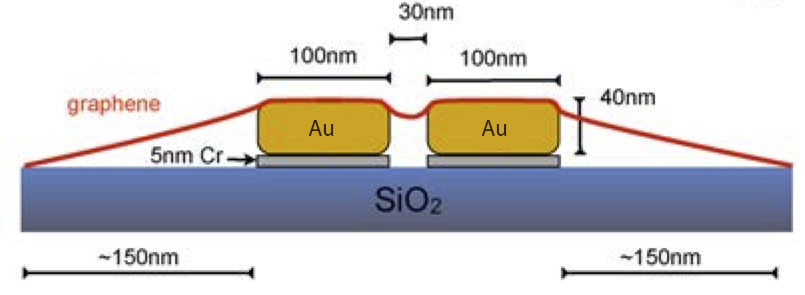
\includegraphics[width=\textwidth]{./images/sers-schema.png}
  \end{subfigure}
  ~
  \begin{subfigure}{0.45\textwidth}
    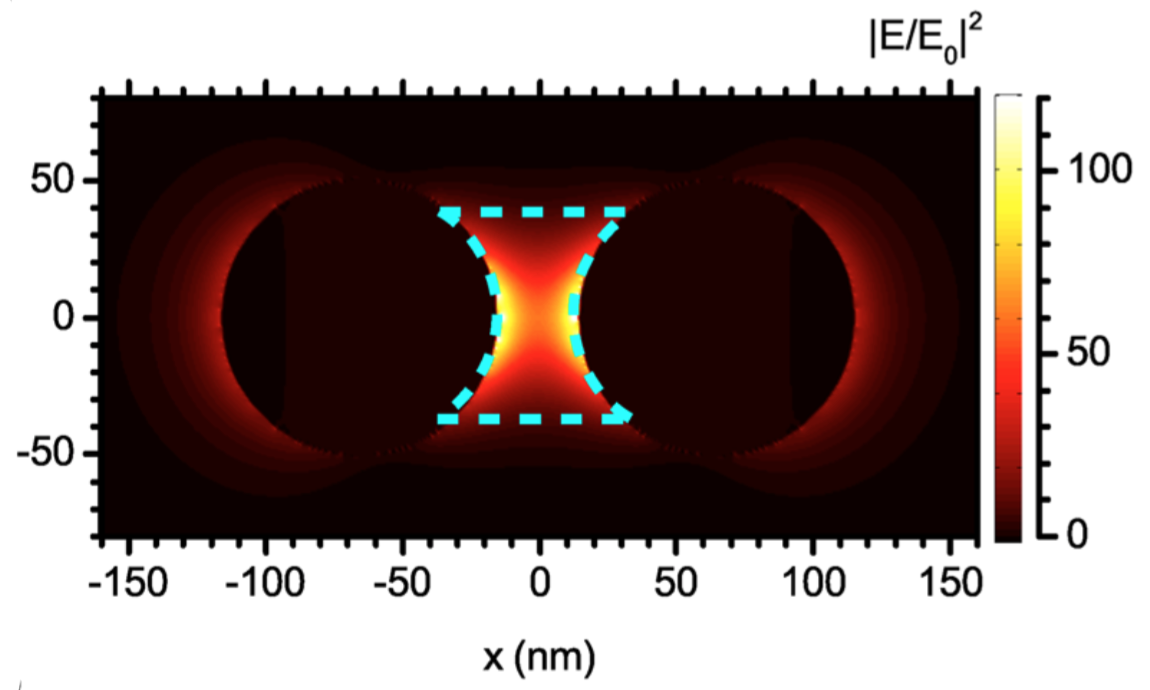
\includegraphics[width=\textwidth]{./images/local-enhancement-heeg.png}
  \end{subfigure}
  \caption{\textbf{(a)} A gold-nanodisk dimer with a chromium interlayer is fabricated with e-beam lithography on a SiO$_2$/Si substrate. A layer of graphene is suspended on top of the nanostructure and pulled into the gap (figure adapted from ref.~\cite{heeg}). \textbf{(b)} Local $\mathbf{E}$-field enhancement at $\lambda = 638nm$ and a distance to the substrate of \SI{40}{nm}. The blue dashed line indicates the area that includes 90\% of the near field intensity according to \cite{heeg} (figure from ref.~\cite{heeg}.)}
  \label{fig:heeg-experiment}
\end{figure}

The experiment relevant for this work is depicted in figure~\ref{fig:heeg-experiment} (for details see ref.~\cite{heeg}). Graphene is suspended on top of two gold disks with a diameter of \SI{100}{nm} and a gap of \SI{30}{nm}. Localized surface plasmons in the gold structures enhance the Raman signal. The near-field intensity enhancement at a distance of \SI{40}{nm} to the substrate is shown in figure~\ref{fig:heeg-experiment}b. The geometry of the nanostructure is chosen to be in resonance with the laser wavelength of $\lambda = \SI{638}{nm}$. Only the component of the electric field that lies within the graphene plane is contributing to the enhancement.

\subsubsection{Electromagnetic-Enhancement Theory of SERS}

The effect of electromagnetic field enhancement actually happens twice in surface-enhanced Raman spectroscopy (SERS): The incoming- and the Raman-scattered light are both enhanced by an interaction with the localized surface plasmon. The local electromagnetic enhancement at position $\mathbf{r}$ and laser frequency $\omega_\mathrm{L}$ can be calculated as\cite{maier2007}
\begin{equation}
  Enh_\mathrm{loc}(\mathbf{r},\omega_L)=\frac{\left|\mathbf{E}_\mathrm{loc}(\mathbf{r}, \omega_L)\right|^2}{\left|\mathbf{E}_0\right|^2}\frac{\left|\mathbf{E}_\mathrm{loc}(\mathbf{r}, \omega_L-\omega_\mathrm{ph})\right|^2}{\left|\mathbf{E}_0\right|^2}\approx\frac{\left|\mathbf{E}_\mathrm{loc}(\mathbf{r}, \omega_L)\right|^4}{\left|\mathbf{E}_0\right|^4},
  \label{eq:enhancement}
\end{equation}
where $\mathbf{E}_\mathrm{loc}$ is the local electric field amplitude, $\mathbf{E}_0$ the electric field amplitude of the reference signal and $\omega_\mathrm{ph}$ the phonon frequency. For a Raman shift that is small compared to the laser frequency, the enhancement is proportional to $\mathbf{E}^4$.
